
% --------------------------------------------------------------
% This is all preamble stuff that you don't have to worry about.
% Head down to where it says "Start here"
% --------------------------------------------------------------

\documentclass[11pt]{article}

\usepackage{bera}
%\renewcommand{\familydefault}{\rmfamily}

\usepackage{graphicx,url}
\usepackage{proof}
\usepackage{framed}
\usepackage{etaremune}

\usepackage[margin=1in]{geometry}
\usepackage{hyperref}
\usepackage{amsmath,amsthm,amssymb,amsfonts}
\usepackage{paralist}
\thispagestyle{empty}

% 1. To get version suitable for students to populate,
%    remove the contents of the \ignoreSoln{..body..}
%
% 2. To get a version suitable for generating PDF 
%    without solutions, remove the #1 below
%
% 3. To generate solutions, keep the #1 below
%
% 4. Assigned grader fills \ignoreSoln{..body..}
%    and also provides his/her feedback to student
%    and policy followed for point deduction
%    So design policy before grading begins.

\newcommand{\ignoreSoln}[1]{#1}   
%\newcommand{\ignoreModel}[1]{#1} 


\newcommand{\bigset}[2]{\big\{\;#1\;:\;#2\;\big\}}
\newcommand{\N}{\mathbb{N}}
\newcommand{\Z}{\mathbb{Z}}
\newcommand{\R}{\mathbb{R}}
\newcommand{\Np}{\mathbb{N^{+}}}
\hypersetup{
    colorlinks=true,
    linkcolor=blue,
    filecolor=magenta,      
    urlcolor=cyan,
    pdftitle={Overleaf Example},
    pdfpagemode=FullScreen,
    }
\newenvironment{theorem}[2][Theorem]{\begin{trivlist}
\item[\hskip \labelsep {\bfseries #1}\hskip \labelsep {\bfseries #2.}]}{\end{trivlist}}
\newenvironment{lemma}[2][Lemma]{\begin{trivlist}
\item[\hskip \labelsep {\bfseries #1}\hskip \labelsep {\bfseries #2.}]}{\end{trivlist}}
\newenvironment{exercise}[2][Exercise]{\begin{trivlist}
\item[\hskip \labelsep {\bfseries #1}\hskip \labelsep {\bfseries #2.}]}{\end{trivlist}}
\newenvironment{reflection}[2][Reflection]{\begin{trivlist}
\item[\hskip \labelsep {\bfseries #1}\hskip \labelsep {\bfseries #2.}]}{\end{trivlist}}
\newenvironment{proposition}[2][Proposition]{\begin{trivlist}
\item[\hskip \labelsep {\bfseries #1}\hskip \labelsep {\bfseries #2.}]}{\end{trivlist}}
\newenvironment{corollary}[2][Corollary]{\begin{trivlist}
\item[\hskip \labelsep {\bfseries #1}\hskip \labelsep {\bfseries #2.}]}{\end{trivlist}}

\DeclareMathSizes{14}{14}{14}{14}

\begin{document}

% --------------------------------------------------------------
%                         Start here
% --------------------------------------------------------------

%\renewcommand{\qedsymbol}{\filledbox}
\newlength{\minpagw}
\settowidth{\minpagw}{\hspace{40em}}

\begin{center}
\begin{large}
  CS 6110, Spring 2022, Assignment 3  \\
  Given 2/3/22 -- Due 2/10/22 by 11:59 pm via your Github 
  \ \\
%  \ \\  
    {  {\Large\bf NAME: Tripti Agarwal} \hfill {\Large\bf UNID: u1319433 }\hspace{4cm} }
          \ \\
\end{large}

\end{center}





\begin{enumerate}
  
%- 1 ----------------------------------------------------------------




    
\item (8 marks) Murphi code \\
\begin{minipage}{\minpagw}
  \fbox{%
    \parbox{\linewidth}{%
      \begin{itemize}
          \item Downloaded rumur and run the make file available on \href{https://github.com/ganeshutah/cs6110s22/blob/master/Lec9/make_rumur.mk}{Github} for the code npretenson.m
         \item Following outputs are obtained for N=3 and 5.
         \begin{itemize}
             \item \textbf{N=3} \\BFS, 35 bits (rounded up to 5 bytes)\\
             172 states, 516 rules fired in 0s.\\
             \item \textbf{N=5}\\
             BFS, 63 bits (rounded up to 8 bytes)\\
             770 states, 33850 rules fired in 0s.
         \end{itemize}
         \item Using sym1 and sym2 flags
         \begin{itemize}
             \item \textbf{N=3, sym1}\\
             BFS, sym1\\
             35 bits (rounded up to 5 bytes)
             172 states, 516 rules fired in 0s
             \item \textbf{N=3, sym2}\\
             BFS, sym2\\
             35 bits (rounded up to 5 bytes)\\
             172 states, 516 rules fired in 1s.
             \item \textbf{N=5, sym1}\\
             BFS, sym1\\
             63 bits (rounded up to 8 bytes)\\
             6770 states, 33850 rules fired in 0s
             \item \textbf{N=5, sym2}\\
             BFS, sym2\\
             63 bits (rounded up to 8 bytes)\\
             6770 states, 33850 rules fired in 0s.
         \end{itemize}
            \item \textbf{N=9}\\
            BFS, sym1 runs for 2871372 states, 25842348 rules fired in 19s.\\
            BFS, sym2 runs for 2871372 states, 25842348 rules fired in 18s.
      \end{itemize}
    }%
 }
\end{minipage}
\newpage
%- 2 ----------------------------------------------------------------
\item (2 points) Photoshop bug\\
\begin{itemize}
    \item To improve the improvement of computation in photoshop, designers adopted parallelism.
    \item Success with parallelism involved basic image-processing routines. This made parallelism involved in the app in a way that did not complicated implementations for the bottleneck-routine algorithms.
    \item This lead to error-prone synchronization primitives. The critical section to enter and leave were very fast in Windows but were highly error prone.
    \item This basically explained how tricky can parallel programming can be. As the cores for the processors increases, the complexity will grow and we need more tools or better programming primitives for hiding the complexity for developers.
    \item As the number of cores increases, the image chunks being processed, called tiles, are sliced into greater number of smaller pieces, resulting in increased synchronization overhead.
    \item The effect the Amdalh's wall, was tried to be fixed by increasing the tile size, which made the sub pieces even larger. Engineers tried fixing it by using another algorithm but it led to memory-bandwidth limitations. This problem caused by the fact that Photoshop cannot interrupt pixel processing operations, until an entire tile is complete.  Hence this will lead to latency issues.

\end{itemize}
\newpage  
%- 3 ----------------------------------------------------------------  
\item (90 points)
\begin{figure}[!h]
\begin{minipage}{\minpagw}
  \fbox{%
    \parbox{\linewidth}{%
      The code had the error in the handle proctype. This can be seen by looking at the cycle in the error trace as shown the figure below:\\
      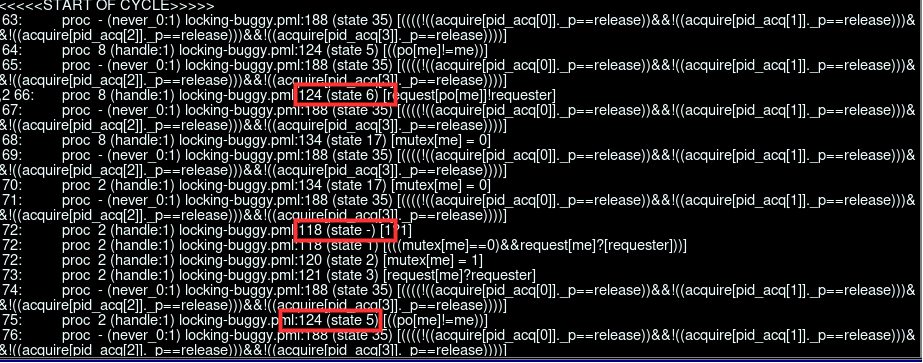
\includegraphics[width = 4.5in]{locking_error.png}\\
      We observe that the cycle is between line 118 and 124. This is because the code in lines 117 to 122 should run once for a particular value of me and then execute line 124 and should loop back to 117. The reason can be seen more clearly from the example, let say po of 2 and 3 is 1. The request channel of 1 consists of 2 and 3. Once the requester is 2 then the handle should make the mutex of po as 1 and 2 should acquire the resources. In the buggy implementation, since the cycle exists, once the requester is 2 it is possible that 3 can also be the requester, and hence we need to stop this issue.
      
      The fix is provided in the code and shown in the snippet below:\\
      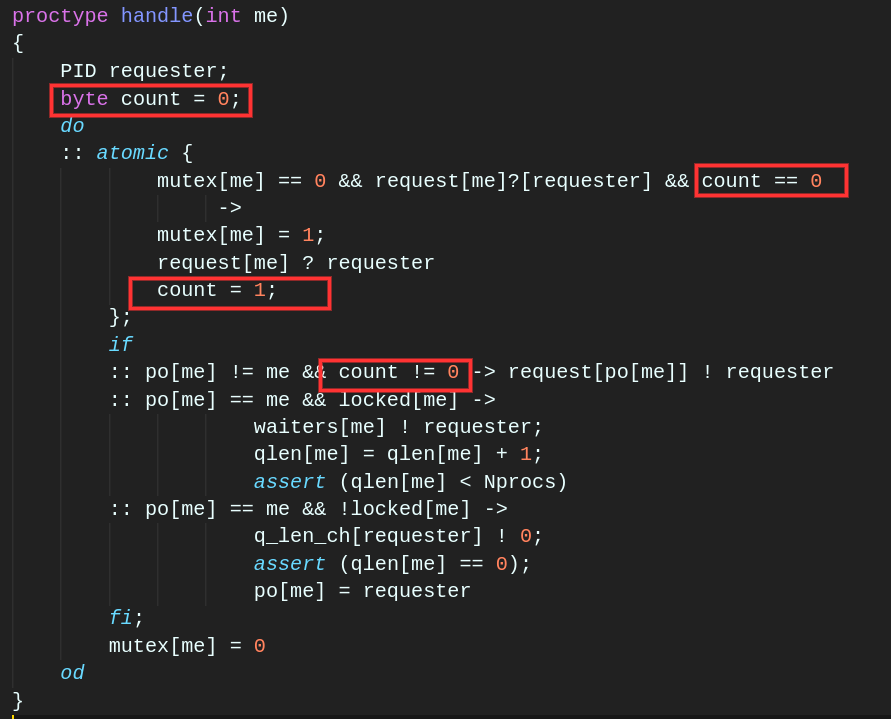
\includegraphics[width=3.5in]{locking_fixed.png}\\
      We see that putting an extra guard of count, which makes the code from line 117 to 122 to run only once and then putting a guard to see whether the code has run that atomic section, resolves the issue and removes the cycle. The output without any error is shown below:
      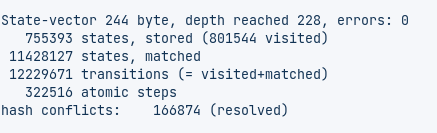
\includegraphics[width=3.0in]{locky_fixed_output.png}
      
    }%
  }%
\end{minipage}
\end{figure}
\end{enumerate}


  
\end{document}
%- end ----------------------------------------------------------------  